%!TEX root = ../../main.tex
\chapter{Installation der PWA}

Dadurch, das die Webanwendung über ein Service Worker und ein Web-Manifest verfügt, kann diese auf dem Endgerät installiert werden. Das von Angular erzeugte Web-Manifest wurde in den Eigenschaften \texttt{theme\_color} und \texttt{backgroud\_color} angepasst, beide Eigenschaften wurden von Blau auf Weiß gesetzt.

Die Installation über Google Chrome erfolgt über den Download-Button in der URL-Suchleiste, siehe Abbildung \ref{img:installChrome}

\begin{figure}[!htb]
    \centering
    \includegraphics[scale=0.7]{installChrome.png}
    \caption{Installation der PWA aus dem Google Chrome Browser durch die Auswahl des Download-Buttons in der URL-Suchleiste des Browsers.}
    \label{img:installChrome}
\end{figure}

Die PWA kann nicht über den Apple Safari Browser auf den Rechner installiert werden. Möchte man die PWA auf einem MacOS system installieren muss somit ein zusätzlicher Browser wie zum Beispiel Google Chrome installiert werden. 

Nachdem die PWA unter Chrome installiert wurde, kann die Applikation unter \textit{Programme} geöffnet werden. Die Desktop-Anwendung der PWA ist in Abbildung \ref{img:desktopPwa} dargestellt.

\begin{figure}[!htb]
    \centering
    \includegraphics[width=\textwidth]{pwaDesktop.png}
    \caption{Die installierte PWA als Desktop-Anwendung}
    \label{img:desktopPwa}
\end{figure}


Wird eine PWA unter Android geöffnet, so wird der Anwender direkt gefragt, ob er diese Installieren möchte, siehe Abbildung \ref{img:installAndroid}.

\begin{figure}%
    \centering
    \subfloat[][]{\includegraphics[width=0.4\linewidth]{installAndroid.png}}%
    \qquad
    \subfloat[][]{\includegraphics[width=0.4\linewidth]{installAndroid02.png}}%
    \caption{PWA installation unter Android}%
    \label{img:installAndroid}
  \end{figure}

Obwohl die Installation eine PWA über Safari auf MacOS nicht möglich ist, kann diese über Safari auf IOS installiert werden. Jedoch müssen hierfür zusätzliche Einstellungen vorgenommen werden. In dem \texttt{head} der \texttt{index.html} muss der Dateipfad zu dem verwendeten Icon angegeben werden, da dieser nicht aus dem Web-App-Manifest ausgelesen wird. 
Des weiteren muss in einem \texttt{Meta-Tag} angegeben werden, dass die Webanwendung als App genutzt werden kann. Diese zusätzlichen Angaben ermöglichen es, die Applikation zu installieren. 
Hierfür kann unter dem \textit{Teilen}-Button die Auswahl \textit{Zum Home-Bildschirm} ausgewählt werden. Nachdem ein Name für die App eingegeben wurde, wird die Anwendung als App zu dem Bildschirm hinzugefügt. In der Folgenden Bilderserien, Abbildung \ref{img:iphone01} bis \ref{img:iphone0n}, sind die einzelnen Schritte aufgezeigt. 

\begin{figure}[!htb]
    \begin{minipage}[b]{.4\linewidth} % [b] => Ausrichtung an \caption
       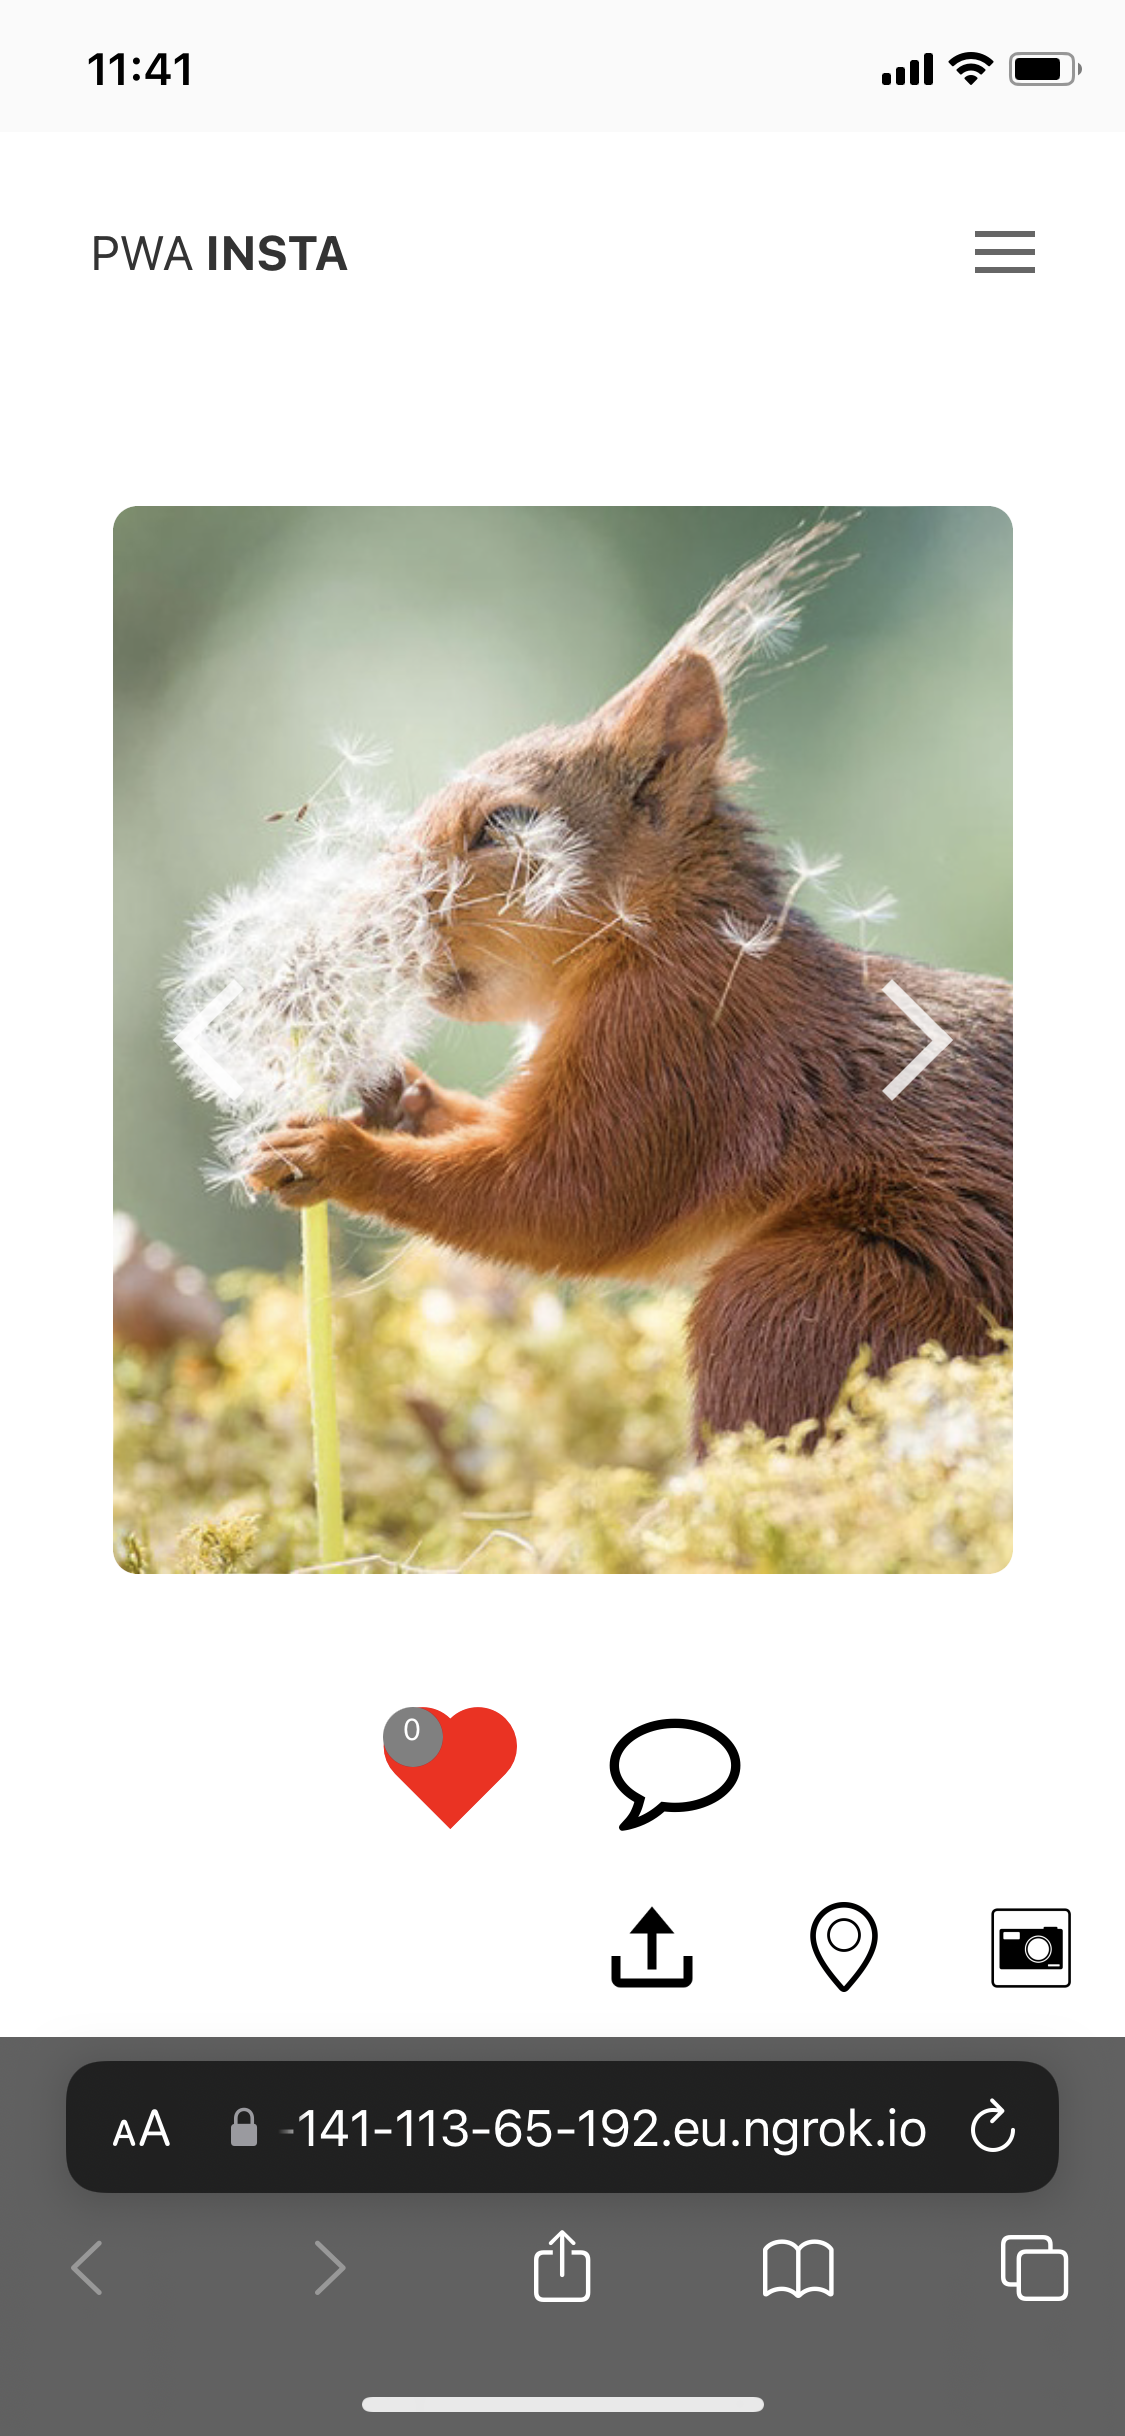
\includegraphics[width=\linewidth]{Iphone01.PNG}
       \caption{PWA im Apple Safari Browser in einem IOS System}
       \label{img:iphone01}
    \end{minipage}
    \hspace{.1\linewidth}% Abstand zwischen Bilder
    \begin{minipage}[b]{.4\linewidth} % [b] => Ausrichtung an \caption
       \includegraphics[width=\linewidth]{iphone02.PNG}
       \caption{Installation der PWA über die Auswahl \textit{Zum Home-Bildschirm}}
    \end{minipage}
 \end{figure}

 \begin{figure}[!htb]
    \begin{minipage}[b]{.4\linewidth} % [b] => Ausrichtung an \caption
       \includegraphics[width=\linewidth]{iphone03.PNG}
       \caption{Eingabe einer Bezeichnung für die PWA-App}
    \end{minipage}
    \hspace{.1\linewidth}% Abstand zwischen Bilder
    \begin{minipage}[b]{.4\linewidth} % [b] => Ausrichtung an \caption
       \includegraphics[width=\linewidth]{iphone09.jpg}
       \caption{Die installierte PWA-App auf dem Home-Bildschirm eines IOS-Systems }
       \label{img:iphone0n}
    \end{minipage}
 \end{figure}


